%%%%%%%%%%%%%%%%%%%%%%%%%%%%%%%%%%%%%%%%%%%%%%%%%%%%%%%%%%%%%%%%%%%%%%%%%%%%%%%%%%%%%%%%%%%%%%%%
%
% CS484 Written Question Template
%
% Acknowledgements:
% The original code is written by Prof. James Tompkin (james_tompkin@brown.edu).
% The second version is revised by Prof. Min H. Kim (minhkim@kaist.ac.kr).
%
% This is a LaTeX document. LaTeX is a markup language for producing 
% documents. Your task is to fill out this document, then to compile 
% it into a PDF document. 
%
% 
% TO COMPILE:
% > pdflatex thisfile.tex
%
% If you do not have LaTeX and need a LaTeX distribution:
% - Personal laptops (all common OS): www.latex-project.org/get/
% - We recommend latex compiler miktex (https://miktex.org/) for windows,
%   macTex (http://www.tug.org/mactex/) for macOS users.
%   And TeXstudio(http://www.texstudio.org/) for latex editor.
%   You should install both compiler and editor for editing latex.
%   The another option is Overleaf (https://www.overleaf.com/) which is 
%   an online latex editor.
%
% If you need help with LaTeX, please come to office hours. 
% Or, there is plenty of help online:
% https://en.wikibooks.org/wiki/LaTeX
%
% Good luck!
% Min and the CS484 staff
%
%%%%%%%%%%%%%%%%%%%%%%%%%%%%%%%%%%%%%%%%%%%%%%%%%%%%%%%%%%%%%%%%%%%%%%%%%%%%%%%%%%%%%%%%%%%%%%%%
%
% How to include two graphics on the same line:
% 
% \includegraphics[\width=0.49\linewidth]{yourgraphic1.png}
% \includegraphics[\width=0.49\linewidth]{yourgraphic2.png}
%
% How to include equations:
%
% \begin{equation}
% y = mx+c
% \end{equation}
% 
%%%%%%%%%%%%%%%%%%%%%%%%%%%%%%%%%%%%%%%%%%%%%%%%%%%%%%%%%%%%%%%%%%%%%%%%%%%%%%%%%%%%%%%%%%%%%%%%

\documentclass[11pt]{article}

\usepackage[english]{babel}
\usepackage[utf8]{inputenc}
\usepackage[colorlinks = true,
            linkcolor = blue,
            urlcolor  = blue]{hyperref}
\usepackage[a4paper,margin=1.5in]{geometry}
\usepackage{stackengine,graphicx}
\usepackage{fancyhdr}
\setlength{\headheight}{15pt}
\usepackage{microtype}
\usepackage{times}
\usepackage{booktabs}
\usepackage{amsmath}

% From https://ctan.org/pkg/matlab-prettifier
\usepackage[numbered,framed]{matlab-prettifier}

\frenchspacing
\setlength{\parindent}{0cm} % Default is 15pt.
\setlength{\parskip}{0.3cm plus1mm minus1mm}

\pagestyle{fancy}
\fancyhf{}
\lhead{Homework Writeup}
\rhead{CS484}
\rfoot{\thepage}

\date{}

\title{\vspace{-1cm}Homework 3 Writeup}


\begin{document}
\maketitle
\vspace{-3cm}
\thispagestyle{fancy}

\section*{Instructions}
\begin{itemize}
  \item Describe any interesting decisions you made to write your algorithm.
  \item Show and discuss the results of your algorithm.
  \item Feel free to include code snippets, images, and equations.
  \item Use as many pages as you need, but err on the short side If you feel you only need to write a short amount to meet the brief, th
  
  \item \textbf{Please make this document anonymous.}
\end{itemize}

\section*{In the beginning...}

 This assignment is could be divided into four parts. First part is converting RGGB images (Bayer pattern) into RGB images using interpolation, bilinear or bicubic methods. Second is using epipolar geometry and eight-point algorithm, deriving the fundamental matrix of given images and data points. Third is using the homography matrices from the fundamental matrix, rectifying two given images onto the common plane and could be easily visualized by stereo anaglyph. The last part is to make cost-volume function using NCC(Normalized Cross Correlation) methods, and to aggregate it using a box filter or in advance use other methods to improve it. 
  
\section*{Interesting Implementation Detail}

 As implementing 'bayer to rgb bicubic.m' in this assignment, I used bilinear method to convert Bayer patterned images, and had to divide all cases in advance, using for-loops in order to handle with exceptions, which is generated for the vertices and sides. As using bilinear method, the most struggling point was to divide the given image into nine pieces, and handling all exceptions, not to pad along the surrounding values.
 
 For calculating the fundamental matrix, applying the normalization method with given points are done by using given function, but it was interesting to transpose the given points to make appropriate calculation. By implementing matrix A, made by crossing around the values of given x, y values of points, getting SVD and erasing the smallest single value to 0, and remultiplying such values helped to get with the fundamental matrix.
 
 To rectify, after moving and tilting the image around with given homography matrices, I had to move the image linearly to align, so that I wanted to use specific points to match them. But it wasn't available to get the movable difference easily, so that I was forced to use pre-calculated values in order to align two different images.

For last, using NCC was also a struggling part, to make the method applicable to various window sizes and max disparity, I also had to divide to 9 cases to handle with all exceptions. From the condition varying by the size of window, as when I cannot get the window as pixel shortage or if maximum disparity was to big enough over the boundaries of canvas. For the lagging case, I handled by zero-ing out the values, while we find the maximum values overall. 

As applying the naive box filter, a 3x3 filter with equivalent elements overall by 1/9, it was useful rather than not using the filter, but I thought up with the Gaussian filter used with other assignments, as seemed to work better using it. 



\section*{A Result}

\begin{enumerate}
    \item As the result of converting bayer filtered image, I successfully converted as Figure  \ref{fig:result1}, as given data points marked as circles alongside the image. 
    
    \begin{figure}[h]
    \centering
    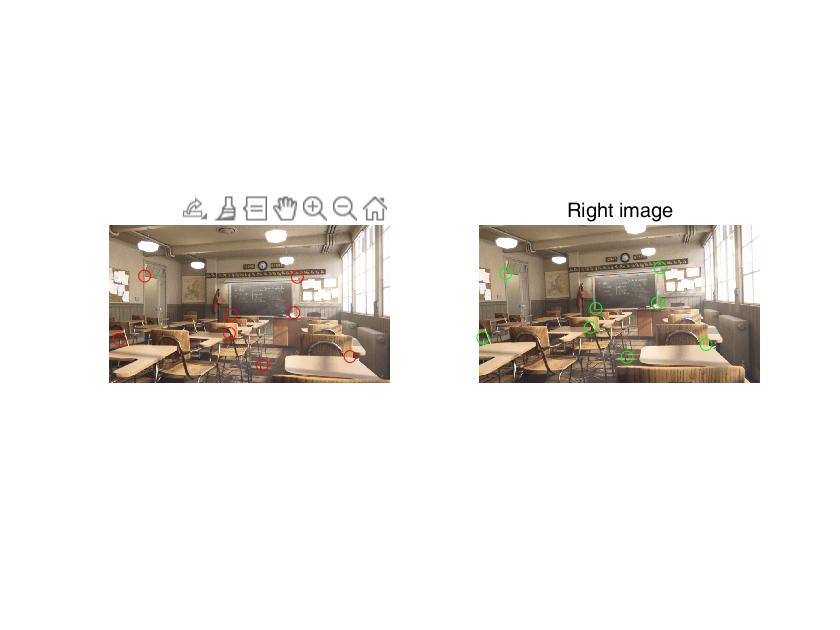
\includegraphics[width=13cm]{figure1.jpg}
    \caption{Left image for image 1, and Right image for image 2}
    \label{fig:result1} 
    \end{figure}
    
    \item By calculating fundamental matrix using given 8 data points for both of the images, I derived 
    the fundamental matrix as 
    
    \begin{equation}
        \begin{matrix}
        3.30225397476813^{-8}& -7.96349124548184^{-7}& -2.38782873327238^{-5}\\
        7.26527864991008^{-7}& -4.10376526640455^{-8}& -0.00462064539929741\\
        -0.000167545047790527& 0.00464905837340531& -0.0214534077223645
        \end{matrix}
    \end{equation}
    
    \item With derived fundamental matrix, rectifying has been done, while tilting the image to a common plane. The results are given as Figure \ref{fig:result2} 

    \begin{figure}[h]
    \centering
    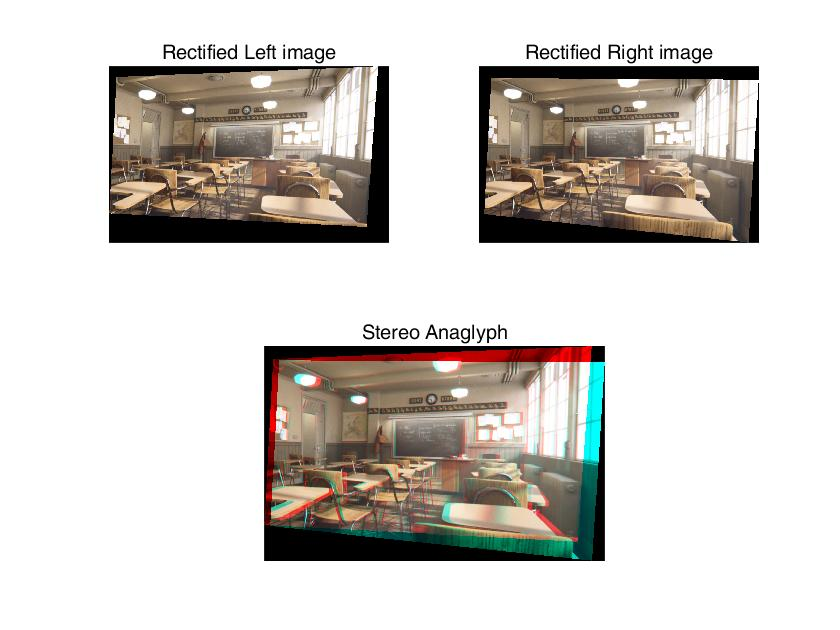
\includegraphics[width=13cm]{figure2.jpg}
    \caption{Left image for Rectified Image 1, and Right image for Rectified Image 2, Bottom center image for the stereo anaglyph for both of the images}
    \label{fig:result2}
    \end{figure}
    
    \item After using NCC methods, I could filter it with Gauissian filter as additional work. These are some photos of disparity map while varying the window size and maximum disparity, as given as Figure \ref{fig:result3}  

    \begin{figure}[h]
    \centering
    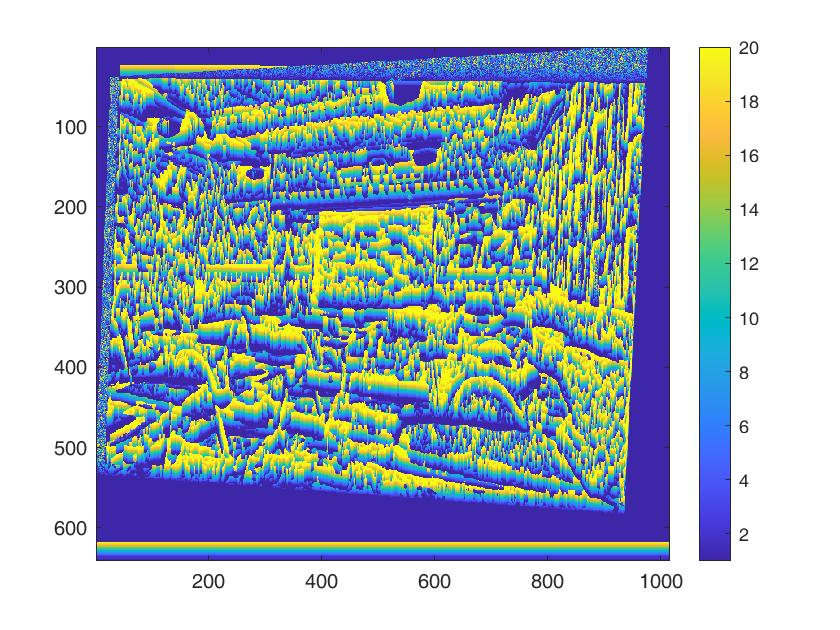
\includegraphics[width=4cm]{figure3_1.jpg}
    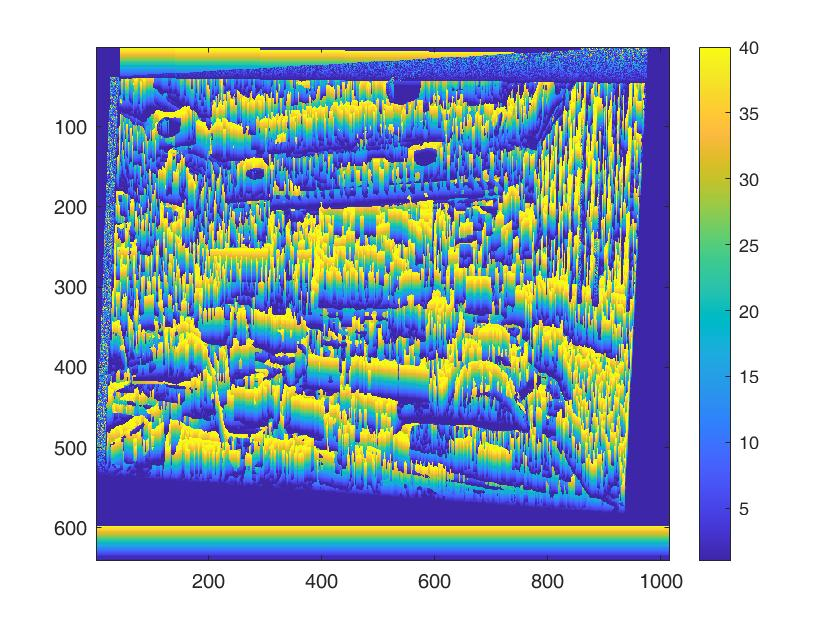
\includegraphics[width=4cm]{figure3_2.jpg}
    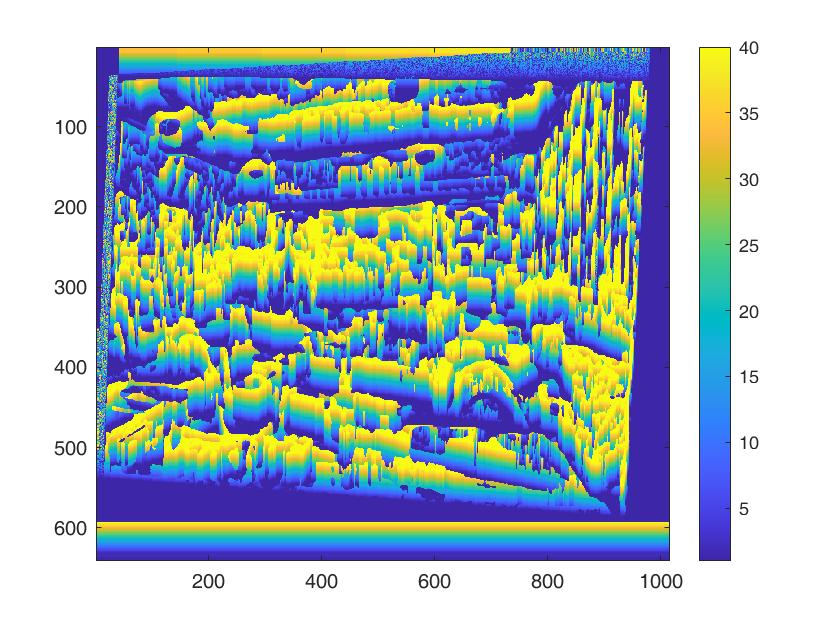
\includegraphics[width=4cm]{figure3_3.jpg}
    \caption{Left image for (5, 20), Middle image for (5, 40) , Right image for (10, 40); (Window Size, Maximum Disparity)}
    \label{fig:result3}
\end{figure}
\end{enumerate}
\end{document}